\documentclass[12pt]{article}

\usepackage[english]{babel}
\usepackage[utf8x]{inputenc}
\usepackage{amsmath}
\usepackage{enumitem}
\usepackage{graphicx}
\usepackage{ulem}
\usepackage{caption}
\usepackage{placeins}
\usepackage[usenames,dvipsnames]{color}
\usepackage[colorinlistoftodos]{todonotes}
\usepackage{listings}
\usepackage{fixltx2e}
\usepackage{scrpage2}
\usepackage{lastpage}
\clearscrheadfoot
\pagestyle{scrheadings}
\usepackage{glossaries}
\usepackage[
top    = 2.75cm,
bottom = 2.00cm,
left   = 2.50cm,
right  = 2.00cm]{geometry}
\setcounter{secnumdepth}{4}


\makeglossaries

\newglossaryentry{soa} {name=SOA, description={Service Oriented Architecture}}
\newglossaryentry{json} {name=JSON, description={Java Script Object Notation}}
\newglossaryentry{rest} {name=REST, description={Representational State Transfer}}
\newglossaryentry{aop} {name=AOP, description={Aspect Oriented Programming}}
\newglossaryentry{oop} {name=OOP, description={Object Oriented Programming}}
\newglossaryentry{bpm} {name=BPM, description={Business Process Management}}
\newglossaryentry{roi} {name=ROI, description={Return of Investment}}
\newglossaryentry{esb} {name=ESB, description={Enterprise Service Bus}}
\newglossaryentry{eai} {name=EAI, description={Enterprise Application Integration}}
\newglossaryentry{erp} {name=ERP, description={Enterprise Resource Planning}}

\begin{document}
\begin{titlepage}
\begin{center}
% Oberer Teil der Titelseite:

\includegraphics[width=0.6\textwidth]{images/logo}\\[1cm]    



\LARGE TGM - HTBLuVA Wien XX \\ IT Department  \\[1.5cm]

% Title
\rule{1.0\textwidth}{1mm}
{ \huge \bfseries \\[0.4cm]  \huge SOA, JSON and REST \\ \LARGE Dezsys-Elaboration \\[0.4cm] }

\rule{1.0\textwidth}{1mm}


% Author and supervisor
\noindent 
\vspace{0.5cm}


\small
\begin{center}
\large
Siegel \textsc{Hannah} \&
Vogt \textsc{Andreas}
\end{center}

% Bottom of the page
{\large \today}
\normalsize
\vfill
\begin{abstract}\noindent This elaboration aims to explain the basic concepts of Service Oriented Architecture and the surrounding impacts of it. Also, REST, JSON and other important standards are discussed. This work was out own work, and all sources have been clearly identified.
\end{abstract}

\end{center}
\end{titlepage}

{\small\tableofcontents}

\printglossaries

%HEADER AND FOOTER
\pagenumbering{arabic}
\ohead{\headmark}
\automark{section}
\ifoot{© Siegel,Vogt}
\ofoot{\pagemark ~of \pageref{LastPage}}

\newpage

\section{General Overview}
\subsection{Services} \label{sec:service}
In order to understand \gls{soa}, an very important concept is a \textit{Service}. \\
\\
\textbf{What is a Service?}\\
%A service can be seen as an Interface which provides a specific function, or as a collection of skills. \cite[page 85]{te} \\
Services (such as RESTful Web services) carry out some small function, such as producing data, validating a customer, or providing simple analytical services.",\cite{searchsoa} \\ The difference between a basic logic and a service is if service-orientation has been applied:
"It's the application of service-orientation design principles that distinguishes a unit of logic as a service compared to other units of logic that may exist solely as objects, components, Web services, REST services or cloud based systems",\cite[page 29]{grau}\\ The patterns and principles which should be applied to a service are discussed in section \ref{sec:dp}. Furthermore, the function of a Service should be clearly defined and very often they are closely related to a business process.  \\\\
\textbf{What does a Service contain of?}\\
A service contains it's functionality, a description of this functionality (section \ref{sec:StandardizedServicecontracts} ) and Basic-operations such as binding, selection, publication or discovery (section \ref{sec:soatriangle}) \cite[page 8]{soagoesreal}. \\
Seen out of an more business related approach, they usually provide clear incident, problem, change, configuration, release, availability and cost management - which helps to gain information and overview the services.\\
Also, a service can contain other services, as closer discussed in section \ref{sec:bpel}
%\textbf{What does a Service contain of?}\\
%"Services are what you connect together using Web Services. A service is the endpoint of a connection. Also, a service has some type of underlying computer system that supports the connection offered. ",\cite{service1} \\ Furthermore, a Service has to have a clearly defined function and very often they should belong to one business process. It can be seen as an Interface which provides a specific function, or as a collection of skills. \cite[page 85]{te}\\ \\
\subsection{SOA}
\textbf{Service-Orientation}\\
Service orientation means, that services of any kind are put into the center of the system, enabling flexible business process (re-)modelling due to a very high business process orientation and loose coupling of the services.\\ \\
\textbf{Service-Oriented Computing}\\
"Service-oriented computing is an umbrella term that represents a distinct distributed computing platform. As such, it encompasses many things, including its own design paradigm and design principles, design pattern catalogs(\cite{patterns}), pattern languages, and a distinct architectural model, along with related concepts, technologies, and frameworks.",\cite[page 22]{grau}\\ \\ 

\begin{figure}[here!]
	\centering
	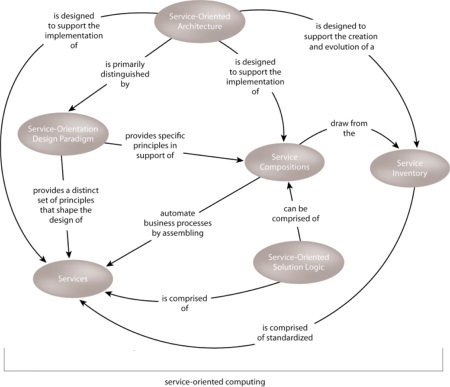
\includegraphics[width=0.7\textwidth]{images/serviceorientationdotcomwhatissoa}
	\caption{Overview of the interactions in Service oriented computing \cite{photos}}
	\label{fig:serviceorientedcomuting}
	\end{figure}
	\FloatBarrier\noindent
\textbf{Service-Oriented Architcture}\\
"Service Oriented Architecture is a technology architectural model for service-oriented solutions with distinct characteristics in support of realizing service-orientation", \cite[page 27]{grau}. \\
As it can be seen in figure \ref{fig:eaipartofso}, historically many components contribute to \gls{soa}. \gls{soa} is often used as a newer approach to \gls{eai}, which is why it may seem quite similar at times.  \cite{soaitwissen} Also, software design principles such as \gls{oop} and \gls{aop} have influenced the design patterns and requirements of \gls{soa}. Furthermore, \gls{bpm} - even trough no software design possibility - has done it's influences into the architecture as well. \\
SOA has it's underlying business functions provided as Services which can be used by all Application on a shared basis. 
\begin{figure}[here!]
	\centering
	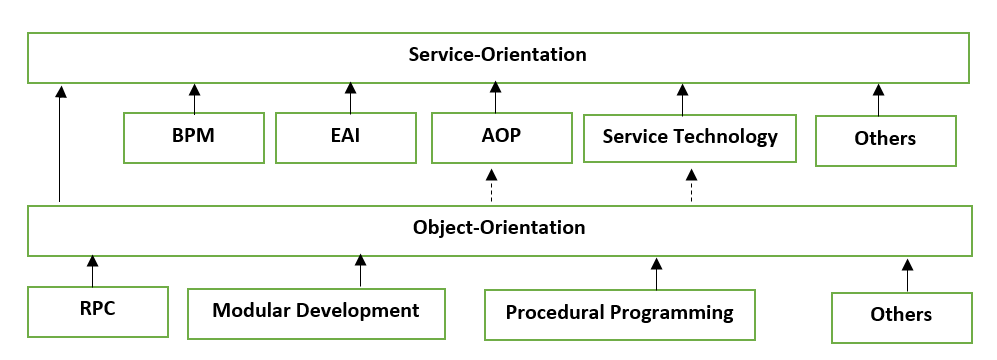
\includegraphics[width=0.8\textwidth]{images/b1_25}
	\caption{Logics that have contributed to SOA (\cite[page 25]{grau}, Hannah Siegel)}
	\label{fig:eaipartofso}
	\end{figure}
	\FloatBarrier
\noindent
%"A service-oriented architecture is essentially a collection of services. These services communicate with each other. The communication can involve either simple data passing or it could involve two or more services coordinating some activity. Some means of connecting services to each other is needed ",\cite{soaserviearch}. \\
%"Service Oriented Architecture is a technology architectural model for service-oriented solutions with distinct characteristics in support of realizing service-orientation", \cite[page 27]{grau}. \\
% Service orientation means, that services of any kind are put into the center of the system, enabling flexible business process (re-)modelling due to a very high business process orientation and loose coupling of the services.\\  \\
%"Service-oriented architecture (\gls{soa}) is an approach used to create an architecture based upon the use of services. Services (such as RESTful Web services) carry out some small function, such as producing data, validating a customer, or providing simple analytical services.",\cite{searchsoa} \gls{soa} is not a product or framework, it is a design approach or paradigm for good software design.
%\\
%SOA has it's underlying business functions provided as Services which can be used by all Application on a shared basis.  \\
%\\ \\
\textbf{Platforms}\\
"It is important to view and position \gls{soa} and service-orientation as being neutral to any one technology platform. By doing so, you have the freedom to continually pursue the strategic goals associated with service-orientation computing by leveragng on-going service technology advancements.",\cite[page 29]{grau} \\ A middleware, such as an \gls{esb} (section \ref{sec:esb}) is used in order to access the services.
\\ \\
\textbf{Success because of \gls{roi}}\\
"One of the keys to SOA architecture is that interactions occur with loosely coupled services that operate independently. SOA architecture allows for service reuse, making it unnecessary to start from scratch when upgrades and other modifications are needed. This is a benefit to businesses that seek ways to \textit{save time and money.}",\cite{searchsoa}. The aspect of an \gls{roi} is very important within the concept of \gls{soa}!
\\ \\\textbf{\gls{soa}'s actors and contributors}\\
\gls{soa} has some important logic components. Next to the in section \ref{sec:service} described Service, which contains of a Service Contract, the implementation and the interface, a service repository and the service bus build the important components without whom \gls{soa} would not be the same. Figure \ref{fig:actorsSoa} provides an overview, which help to understand the basic concepts. The service repository is explained in section \ref{sec:soatriangle}.
	\begin{figure}[here!]
	\centering
	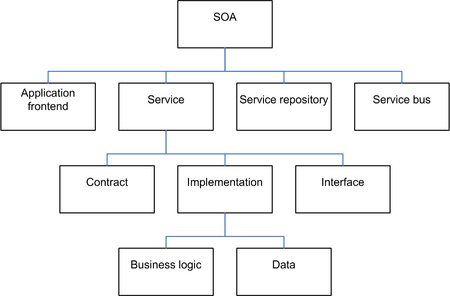
\includegraphics[width=0.7\textwidth]{images/arg2}
	\caption{Overview of the actors in SOA \cite{arg2}}
	\label{fig:actorsSoa}
	\end{figure}
	\FloatBarrier
	\newpage
\subsection{REST}
Rest stands for REpresentational State Transfer. It is a software architecture style consisting of guidelines and best practices 
for creating scalable web services.The main idea behind REST is that you are working with the HTTP protocol. Rest is basically using HTTP verbs, GET, POST, PUT, DELETE and HEAD, in order to act on resources,represented by individual URIs(Uniform Resource Identifiers). 
A perk of those verbs is that they are mostly self-explanatory. REST is a lightweight alternative to mechanisms like RPC (Remote Procedure Calls) and Web Services (SOAP, WSDL, etc. ). \\
REST-based architectures are built from resources (pieces of information) that are uniquely identified by URIs. For example, in a RESTful purchasing system, each purchase order has a unique URI.
REST components manipulate resources by exchanging representations of the resources. For example, a purchase order resource can be represented by an XML document. Within a RESTful purchasing system, a purchase order might be updated by posting an XML document containing the changed purchase order to its URI.
An code example for WSDL can be found in section \ref{sec:wsdlexample}, 
and a code example for SOAP can be found in section \ref{sec:soapexample}
\subsection{JSON}
"JSON (JavaScript Object Notation) is a lightweight data-interchange format. It is easy for humans to read and write. It is easy for machines to parse and generate. It is based on a subset of the JavaScript Programming Language, Standard ECMA-262 3rd Edition - December 1999. JSON is a text format that is completely language independent but uses conventions that are familiar to programmers of the C-family of languages, including C, C++, C sharp, Java, JavaScript, Perl, Python, and many others. These properties make JSON an ideal data-interchange language.",\cite{json}.\\
An comparison between JSON and XML can be found in section \ref{sec:json}.
\section{Existing Problems}
\subsection{Historical Overview}
%With the rise of computers, companies have started to invest into the new information technology during the second half of the 20 century.  Mostly, the first thing that has been bought were expensive mainframes, so that some processes could be done with more reliability. Naturally, employees have done some faults and they were not as efficient as computers. \\
%Because of very expensive Hardware and Software which was by far not as evolved as it is today, the implementation of new technologies was quite slow. Computers and Mainframes were mostly used for industries like astronautics or applied researching and eventually even for automating processes such as book keeping. \\ 
%These implementations were quite easy to implement and there was no need for any intercommunication between services.
%\\ \\
%In the early 80s, the whole industry changed. Suddenly, the personal computer (PC) made it possible to afford information technology on a large scale. Computers were not only used for difficult arithmetic operations but they started to be an everyday-life tool to improve the work-flow and the business processes in companies. \\
%Many new kinds of technologies, ranging from OS with GUIs to the rise of the World Wide Web, were leading to an really fast expansion of information technology. \\ 
%But with an higher demand on PCs, the demand for infrastructure rose as well. The need for computer specialist was higher than ever and every company had to invest a lot into their, mostly newly founded,  IT department. \\ \\
%Because of an lack of know-how and systems that had the characteristics to change a lot, the implementation of all the services became a big challenge. Enterprises used a variety of customised applications, at least one for every type of service. \\ \\
%\textbf{ODER:}
"Historically, many IT projects focused solely on building applications designed specifically to automate business process requirements that were current at that time. This fulfilles immediate (tactical) needs, bit as more of these single-purpose applications were delivered, it resulted in an IT enterprise filled with islands of logic and data referred to as application \textit{silos}. As new business requirements would emerge, either new silos were created or integration channels between silos were established. As yet more business change arose, integration channels had to be augmented, even more silos had to be created, and soon the IT enterprise landscape became convoluted ad increasingly burdensome, expensive, and slow to evolve."\cite[page 522]{grau} 
\subsection{Problems}
Out of these systems, there are many problems that have eventually emerged:
\\ \\\textbf{Resistant to change}\\
First of all, systems like these are not really agile. Because changes and new technologies were inevitable, time consuming integrations had to be done. If these integrations were not done, legacy systems emerged. These were often not remotely changeable as they are with \gls{soa}. \\
Also, new challenges such as cloud computing and a more common globalization of processes made it harder to stick to the old systems in the last view years. \\
Because applications were always providing some kind of service or functionality, but hardly seen like a service, they were not as easy reconfigurable and changeable. \\
\\ \\\textbf{Communication and data transmission}\\
All the applications need to communicate with each other and transmit data, so often a start topology was used. It then changed more and more into a Middle-ware with the upcoming of \gls{eai}, which had the benefit of only docking the Application to the Middle-ware once. Nowadays, mostly a bus system gets used (section \ref{sec:esb}), what makes it a lot easier to communicate in a heterogeneous environment. \\
\\ \\\textbf{Vendor dependency}\\
Due to compatibility concerns, IT-Infrastructures were often Vendor dependent. Therefore we often talk about an SAP-System, because mostly all the components have been bought from SAP, which decreases the agility and may increase the costs.\\
\\ \\\textbf{No support to \gls{bpm}}\\
Furthermore, Applications were not divided into processes, and therefore \gls{bpm} was made difficult to realize for both the management and the IT-department. \\ \\
All these restrictions lead to increased overall costs and an reduced \gls{roi}.
\section{SOA as the solution} 
"In many ways, service-orientation emerged in response to these problems. It is a paradigm that provides an alternative to project-specific, silo-based, and integrated application development by adamantly prioritizing the attainment of long-term, strategic business goals.",\cite[page 522]{grau} \\
The target state of service-orientation is to not have these traditional problems any more. In some cases, due to legacy systems or other problems this is not possible, but still \gls{soa} tries to realize it to whatever extend possible.
\\ \\
Service-orientation emerged as a formal method in support of achieving the following goals an benefits associated with service-oriented computing: \\
\begin{itemize}
\item Increased Intrinsic Interoperability
\item Increased Federation
\item Increased Vendor Diversification Options 
\item Increased Business and Technology Alignment
\item Increased \gls{roi}
\item Increased Organizational Agility
\item Reduced IT Burden
\end{itemize} \cite[page 23]{grau}\\
As it can be seen in figure \ref{fig:goalssoa}, an increase of interoperability,  business and technology alignment, federation and vendor diversification options automatically lead to a increase of the \gls{roi}, the organizational agility and to an reduced IT burden.
\begin{figure}[here!]
	\centering
	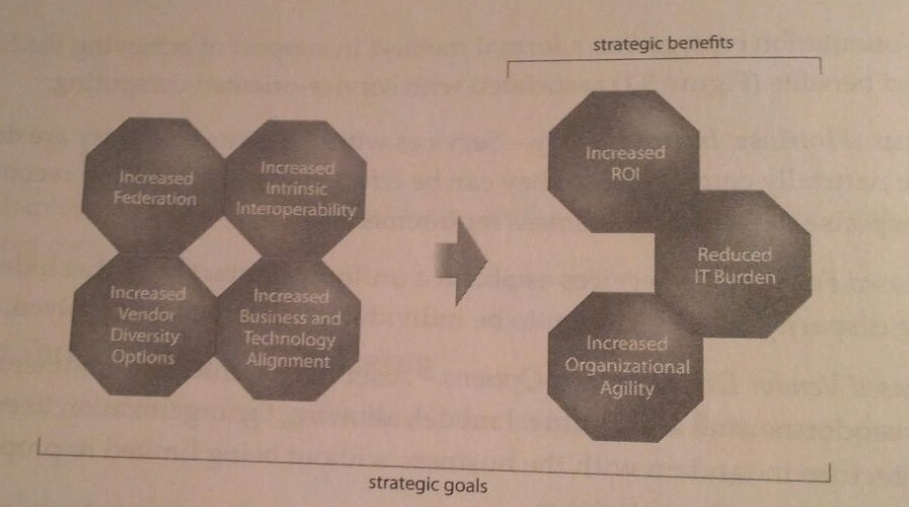
\includegraphics[width=0.6\textwidth]{images/page24}
	\caption{Goals of SOA\cite{photos}\\ SOA Principles of Service Design, (c) Prentice Hall/PearsonPTR}
	\label{fig:goalssoa}
	\end{figure}
\FloatBarrier
 \noindent
These goals are especially interesting not only to IT-staff members but also for a organization's management. \\
These strategic goals the are put into more low-level design principles.

\subsection{Design Principles}
\label{sec:dp}
Because SOA is only an Design Paradigm and not a concrete implementation, service orientation Patterns and principles are used.\\\\
These principles emerged from the theory in software engineering, Separation of Concerns, which means that a problem can be solved easier if divided into smaller parts. This enables to separate a problem into smaller units, and they can then be reused, composed and managed more flexible.  \cite[page 86]{te}\\ Furthermore, they emerged out of all the principles and design considerations that have formed \gls{soa} itself.
\\
These paradigms are often already used in \gls{oop}, and they often cohere. For example, if a system is loosly coupled, it automatically comes with more flexibility which therefore helps the service autonomity. \\
Also, it is not always possible to perfectly achieve all the requirements, so when implementing \gls{soa}, these design principles should be used at the \textit{most possible extend}, but we still speak of \gls{soa} even if not all the rules apply to 100\%. \\ \\
The design paradigm consists of the following points:
\begin{enumerate}
\item Standardized Service contracts
\item Loosly coupled systems
\item Abstraction of Services
\item Service Reusability
\item Service Autonomity
\item Service Statelessness
\item Service Discoverability
\item Service Composability
\end{enumerate}\cite[page 25]{grau}\\
The following discussed principles can be found on searchsoa.com(\cite{photos}) as well, where they are discussed much more in detail.\newpage
\subsubsection{Standardized Service contracts}
\label{sec:StandardizedServicecontracts}
"A service contract expresses the technical interface of a service. ", \cite[page 33]{grau}. This means that there are interfaces which do contain the metadata to an service, as well as describing their functionality, their Datatypes and rules of actions. \cite[page 86]{te} \\ If these services are implemented as a Webservice, for example, most commonly an description document in Form of an WSDL definition will be used, or an XML Schema. \\
The two approaches nowadays are either Top-Down (designing the service contracts at first and then implementing the service) or Bottom-up(Building the contracts out of already existing services). \cite[page 151,152]{grau}
\begin{figure}[here!]
	\centering
	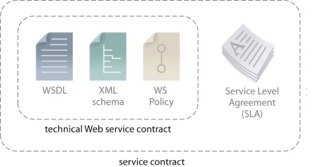
\includegraphics[width=0.49\textwidth]{images/soajuhu}
	\caption{Components of a Service contract \cite{photos}}
	\label{fig:servicecontractcomponents}
	\end{figure}
\FloatBarrier
 \noindent\textit{Service Level Agreements} \\
Furthermore, A service contract will often be concluded in Human Readable documents. These are called Service Level Agreements (SLAs) and they often contain information like quality requirements or overall business information. 
\\ \\
\textit{Service Contract Generation Possibilities within Java} \\
WSDL documentation or service skeletons can be gernerated in Java:\\ 
"JAX-WS defines the wsimport tool, which takes an existing WSDL definintion as input to generate Java skeletons [..] Similarly, the wsgen tool generates WSDL from existing Java code.",\cite[page 151]{grau}
 \noindent\textit{REST}\\
"For REST services, capturing and communicating various aspects of resources can be necessary, such as the set of resources, relationships between resources, HTTP verbs allowed on resources and supported resource representation formats. Standards such as WADL(Web Application Description Language), can be used to satisfy the mandatory requirements. [..] Even the self-describing contract of HTTP verbs for a REST service establishes a standard-based service contract.", \cite[page 151]{grau}
\subsubsection{Loosly coupled systems}
Coupling describes the relationship between two and more things. Loose coupling, a well known design principle,  tries to minimalize the relationships between a service and other components. \cite[page 87]{te} \\
"Loose coupling is an approach to interconnecting the components in a system or network so that those components, also called elements, depend on each other to the least extent practicable. Coupling refers to the degree of direct knowledge that one element has of another", \cite{loosecoupldef}.\newpage
\subsubsection{Service Abstraction}
Abstraction, as a well known design principle in object orientation, means that internal details or workflows of a logic block should be hidden, in order to gain more flexible and loosely coupled systems. \cite[page 87]{te} For example, abstraction would be an abstraction into an API.\\
"The appropriate level of abstraction at which services are described achieves additional agility and alignment between business and IT areas of an enterprise. Abstracting information means taking technical details out of a problem to be solved on a higher level"\cite[page 184]{grau}\\\\
"Service-orientation continues the evolution of higher-level abstraction use to make creating and changing solutions easier."\cite[page 184]{grau}
\subsubsection{Service Reusability}
Reusability, as one very important design principle within the whole software engineering world, has the possibility to become even more powerful when using \gls{soa}, due to the combination with the other design principles applied. \\  Because services are already designed to be reusable, not dependent and stateless, they can be combined really easy. This is again achieving a extend of reusability that has never been possible before. Also, the possibility to regain information about which service or functionality is already available in the design phase more easily (see section \ref{sec:disc}) trough the service inventory helps with the composability of a service. \cite[page 87-88]{te}
%The following are common design characteristics associated with reusable services:
%\begin{itemize}
%\item The service is defined by an agnositc functional context \\
%	This means that an agnostic functional context is not specific to any one purpose and is therefore considered %muli-purpose. It means, that it is idependent of the particular business process or the area of application.
%\item The service logic is highly generic %TODO ???
%\item The service can be used concurrently
%\end{itemize}
\subsubsection{Service Autonomy}
"Service-orientation revolves around building flexible systems. Flexibility is, to a large degree, archived through making services decoupled and autonomous to enable them to be composed, aggregated and changed without affecting other parts of the system. For a service to be autonomous, the service must be as independent from other services with which it interacts, both functionally and from a runtime environment perspective. Java and Java EE provide a highly efficient runtime environment that supports service composition. For example, a Java EE application server support concurrent access to its hosted components, making each access to such a component autonomous from the others.", \cite[page 194]{grau}\\\\
Also, a service's level of autonomy depends on how much control a service has over it's resources, and it promotes the availability and the reliability of a service as well. \cite[page 88]{te}
\subsubsection{Service Statelessness}
If too many states of a service must be managed, scalability and reliability will suffer. Therefore, a service should be designed in a way that it does not need to keep any state as far as possible. \cite[page 88]{te}\\
This means that: "each invocation of a service operation is completely independent from any other invocation, whether by the same consumer or any other service consumer. The service statelessness principle offers various benefits centered around improved scalability by which additional stateless service instances can be easily provisioned on available environments.", \cite[page 197]{grau}\\
\\
"Many real-life business scenarios can be expressed as business processes that include automated steps, which can require manual intervention. Designing and implementing such a process requires some state to be maintained for the duration of the process. Executing an instance of the process definition forms the notation of a session or transaction across multiple service invocations. Therefore, a service implementing the execution of a business process cannot be stateless and may need to even maintain context information over extended periods",\cite[page 197]{grau} This means, that statelessness is probably the hardest design principle to achieve.
\subsubsection{Service Discoverability}
\label{sec:disc}
"The two primary aspects of the Service Discoverability principle are discovery at design-time (which promotes service reuse in a newly developed solution), and discovery at runtime (which involves resolving the appropriate endpoint address for a given service or retrieving other metadata).", \cite[page 204]{grau}\\These two enable a dynamic reuseability of a service, increasing therefore the \gls{roi}. This design principle is often implemented using a service registry. \cite[page 89]{te} \\\\
\noindent\textit{Design-Time Discoverability}\\
"At design-time, it is important for project teams to be able to effective identify the existence of services that contain logic relevant to the solution they plan to build. This way they can either discover services that they can reuse or confirm that new service logic they plan to build does not already exist. For example, a service is designed to address an Order Management business process for which customer information is required. The service designer mist investigate whether a \texttt{Customer} data type already exists and if so deterine whether it meats the requirements for the Order Management Process service." \cite[page 204-205]{grau}\\\\
\textit{Run-Time Discoverability}\\
"Runtime service discovery refers to the ability of software to programmatically search for services using APIs exposed by the service registry. Doing so allows for the retrieval of the physical location or address of services on the network. Because services may need to be moved from one machine to another or perhaps redundantly deployed on multiple machines, it may be advisable for service addresses not to be hardcoded onto the service consumer logic. [..] In addition to the lookup of a service endpoint address, other artifacts can be used by service consumers at runtime to identify an appropriate service and build the applicable request message. The JAX-WS Dispatch API allows a service request to be completely built at runtime."\cite[page 205-207]{grau}
\subsubsection{Service Composability} 
"The composability of a service is an implicit byproduct of the extend to which the other service-orientation design principles have been successfully applied. [..] For example, a service contract that is standardized allows interaction and composition between services implemented in different languages using different runtime environments."\cite[page 189]{grau}\\
Services must be able to be part of any composition, regardless if they were meant to take part at a certain one at the time they were build. \cite[page 89]{te} \\
The composability can be seen in figure \ref{fig:composserv}, where Service B, C and D are using service A, but Service A can also be used independently.

\begin{figure}[here!]
	\centering
	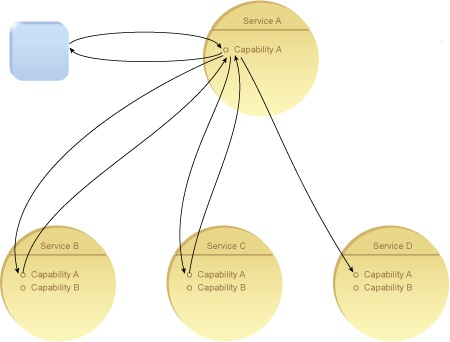
\includegraphics[width=0.49\textwidth]{images/serivceorientationdotcom}
	\caption{Composing of services \cite{photos} \\ SOA Principles of Service Design, (c) Prentice Hall/PearsonPTR}
	\label{fig:composserv}
	\end{figure}
\FloatBarrier
 \noindent
\subsection{Interoperability}
When doing research on \gls{soa}, the principle of interoperability is often named, but it is not part of the official design principles named in section \ref{sec:dp}. This is because interoperability, which means the principle of services working together in order to achieve a bigger functionality, is already secured by the other design principles. It these principles were applied at a meaningful extends, interoperability is automatically provided, and it is fundamental to the success of \gls{soa}.\\
For example, service contracts are standardized so through it's coordination of datamodels interoperability is assured. If the level of coupling is reduced, interoperability is increased, because a call of a service depends on less dependencies. Also, reusability helps a lot in order to achieve interoperability. \cite[page 89-90]{te}
\newpage
\subsection{SOA Manifesto}
The \gls{soa} Manifesto has been developed 2009, and it is quite similar to the Agile Manifesto, which is widely known. Of the Value-Groups, both values are important and should be archived, but the left one is always more important. \\ \\
\textbf{The wording of the SOA Manifesto:}\\ \\ 
"We have been applying service orientation to help organizations 
consistently deliver sustainable business value, with increased agility
and cost effectiveness, in line with changing business needs. \\ \\
Through our work we have come to prioritize: \\
\begin{itemize}
\item Business value over technical strategy 
\item Strategic goals over project-specific benefits 
\item Intrinsic interoperability over custom integration 
\item Shared services over specific-purpose implementations 
\item Flexibility over optimization
\item Evolutionary refinement over pursuit of initial perfection
\end{itemize}" \cite{soamaifesto}
\subsection{SOA Lifecycle}
"As is true of service-oriented architecture (SOA) itself, the SOA lifecycle is a wide-ranging topic and even experts differ in their definition of it and the areas they believe need to be emphasized.",\cite{soalycman}.\\\\
What differentiates the SOA lifecycle from the traditional application lifecycle, is the need for governance to maintain order with loosely coupled services.\cite{soalycman}
\\
The SOA lifecycle stretches all the way from understanding context, including enterprise architecture and business architecture, through service analysis and modeling. And that modeling isn't just about functional issues, it's also about non-functional issues such as security, performance, auditing and so on. Then there is development, testing, provisioning, monitoring and change management. \cite{soalycman}\\
The challenge with the SOA lifecycle is that there are essentially two different lifecycles going on, that overlap. On the one hand there is still the traditional software lifecycle where services are interfaces to running software. But then you also have the service lifecycle (figure \ref{fig:Servicelifecycle}) and that takes place at the metadata level.\\
As services are updated, composed or reconfigured in the software level, the real goal is to do all the changing at the metadata level."\cite{soalycman}\\
\\
%With SOA, you're talking about two different types of applications you're building. The first one you're building is the service that is a completely self-contained unit that does a specific thing such as 'return value of bank account.' So there's one lifecycle (figure \ref{fig:Servicelifecycle}) for that service and another lifecycle that applies to compositing that and other services into a final application. \cite{soalycman} \\
%\\
\\
\textbf{SOA Lifecycle defined by \cite{soalycman}}
\begin{enumerate}
\item Data collection including gathering of business requirements and use cases
\item $\Longrightarrow$ Design including determining service requirements, setting service policies, establishing compliance tasks
\item $\Longrightarrow$building and testing models, and constructing data integration
\item $\Longrightarrow$Development including developing the service and composing the application from the services 
\item $\Longrightarrow$QA/Test/Acceptance  
\item $\Longrightarrow$Deployment 
\item $\Longrightarrow$Monitoring/management 
\item $\Longrightarrow$Change 
\item $\Longrightarrow$Retirement 
\end{enumerate}
	
\begin{figure}[here!]
\centering
\begin{minipage}[h]{0.3\textwidth}
\centering
    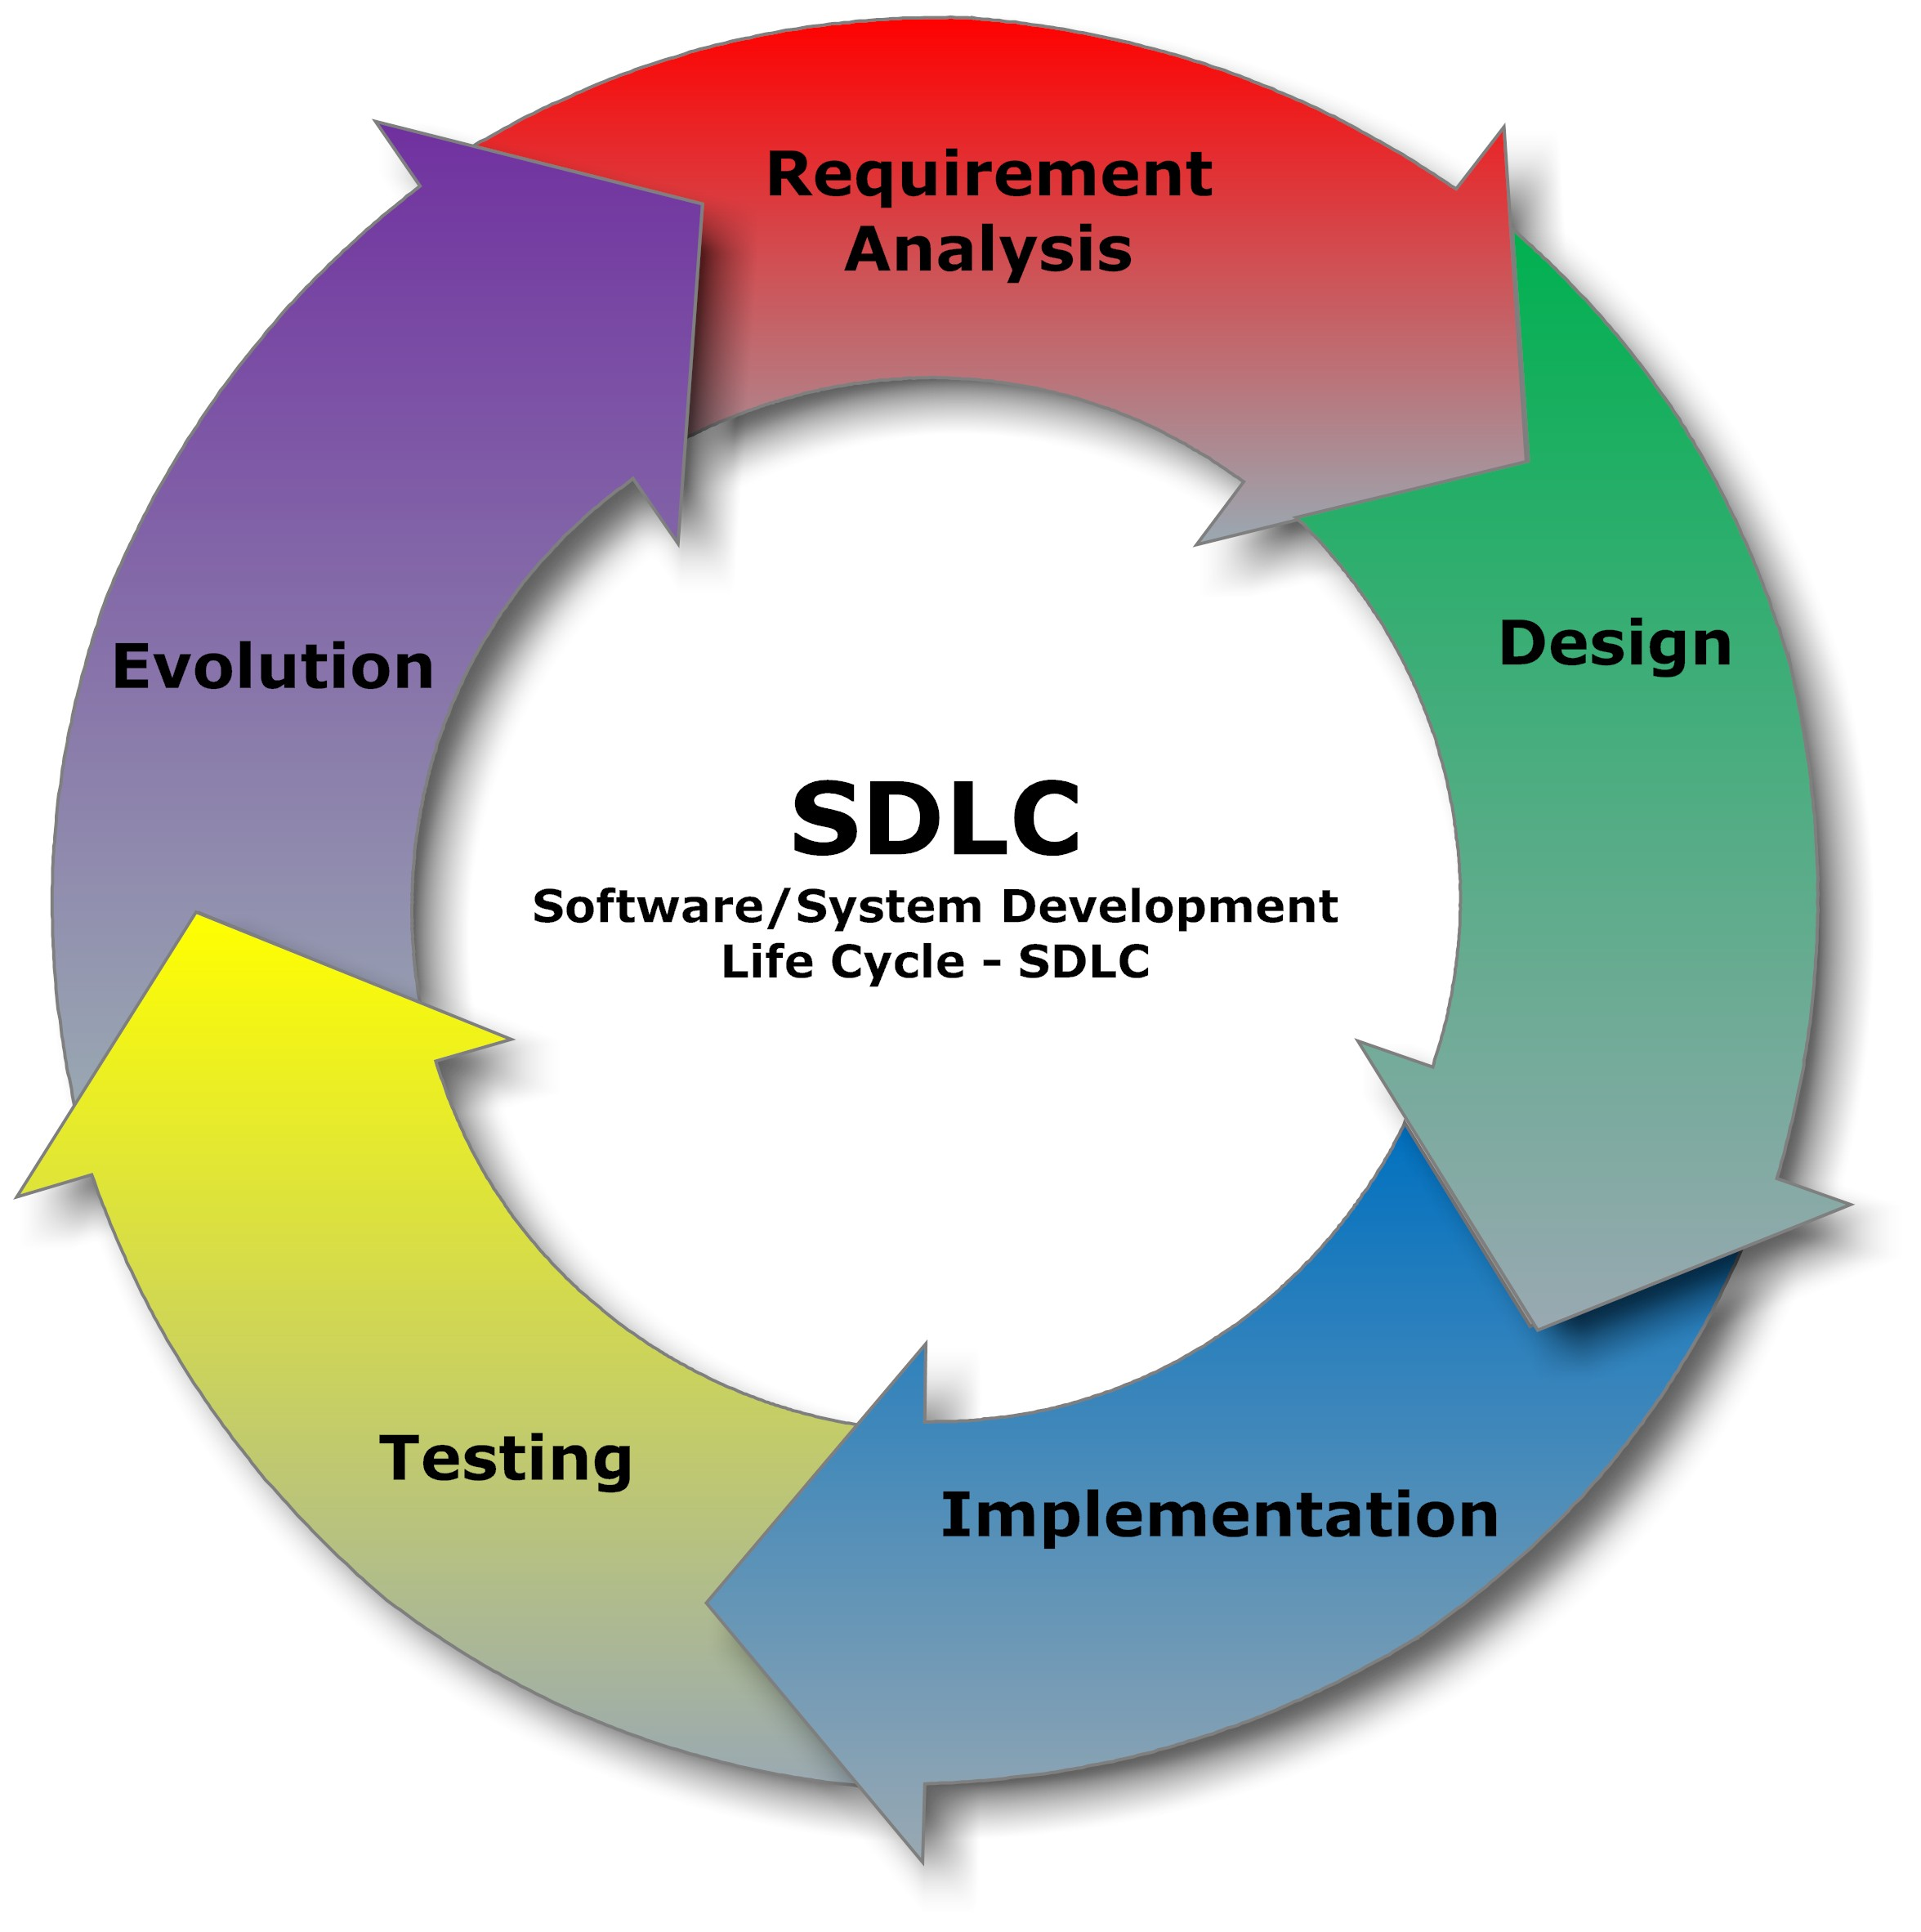
\includegraphics[width=1.0\textwidth]{images/sdlc}
    \caption{Normal Software Development cycle \cite{muede2}}
    \label{fig:asdas}
\end{minipage}
\begin{minipage}[h]{0.14\textwidth}
\vfill
\end{minipage}
\begin{minipage}[h]{0.55\textwidth}
\centering
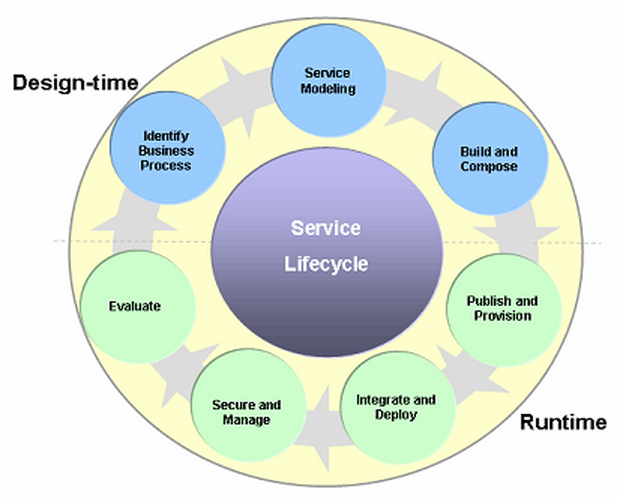
\includegraphics[width=1.0\textwidth]{images/scly.png}
	\caption{Service lifecycle \cite{slcmoracle}}
	\label{fig:Servicelifecycle}
\end{minipage}
\end{figure}
\FloatBarrier	
	%TODO eine section??? 
\newpage
\subsection{BPM}
BPM stands for Business Process Management and this is a systematic approach to make an organisation's workflow more effective, more efficiant and more capable of adapting to an ever-changing environment. 
\\ \\\textbf{What is a business process?}\\
"A business process in an activity or an set of activities that will accomplish a specific organisational goal. The goal of BPM is to reduce human error and miscommunication and focus stakeholders on the requirements of their roles. BPM is a subset of infrastructure management, an administrative area concerned with maintaining and optimizing an organization's equipment and core operations.", \cite{bpmdef}.
\\ \\\textbf{What has BPM to do with SOA?}\\
The Business Process level is very important to every service-oriented architecture, as it is seen as the higher-level controlling instance. Service composition and Orchestration are helping to ensure a business process remodelling is made easy and failure-tolerant at any time. \cite[page 114]{te}
\begin{figure}[here!]
	\centering
	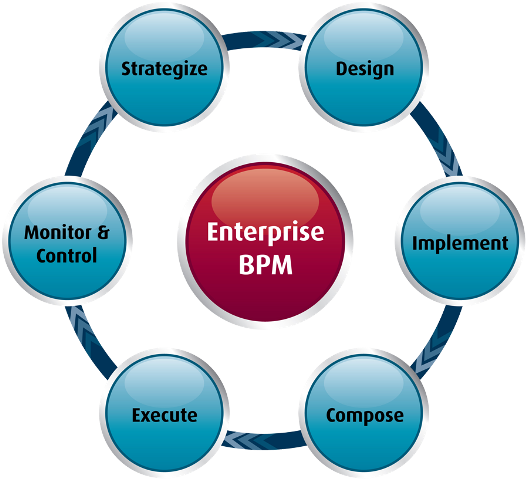
\includegraphics[width=0.5\textwidth]{images/bpm.png}
	\caption{Business Management lifecycle \cite{muede2}}
	\label{fig:anfang}
	\end{figure}
	\FloatBarrier \noindent
\textbf{Challenges of BPM \cite{bpmchall}}
\begin{itemize}
\item Lack of Business Case
\item Too Slow to React to the Business Change
\item Gap between the modelling and the implementation phases
\item Seen as a One Time Project 
\item Not Investing in Staff
\item Poorly Defined Measures of Success 
\end{itemize}
\textbf{BPML and BPQL} \\
"Business Process Modeling Language (BPML) is an Extensible Markup Language (XML)-based metalanguage developed by the Business Process Management Initiative (BPMI) as a means of modeling business processes. [..] BPML 0.4 includes specifications for transactions and compensating transactions, dataflow, messages and scheduled events, business rules, security roles, and exceptions. \\ An associated query language, Business Process Query Language (BPQL) has been developed as a standard management interface that can be used to deploy and execute defined business processes. According to BPMI, BPML and BPQL will be used to establish a standardized means of managing e-business processes through Business Process Management Systems, similarly to the way that SQL established a standardized means of managing business data through packaged database management systems.", \cite{bpmldefmr}
\subsubsection{Orchestration using BPEL}
\label{sec:bpel}
"BPEL (Business Process Execution Language) is an XML-based language that allows Web services in a service-oriented architecture to interconnect and share data.",\cite{bpelsearchsoa}. When using Webserivces, it also is often called WSBPEL. "Programmers use BPEL to define how a business process that involves web services will be executed. BPEL messages are typically used to invoke remote services, orchestrate process execution and manage events and exceptions.\\
BPEL is often associated with Business Process Management Notation (BPMN), a standard for representing business processes graphically. In many organizations, analysts use BPMN to visualize business processes and developers transform the visualizations to BPEL for execution.\\
BPEL was standardized by OASIS in 2004 after collaborative efforts to create the language by Microsoft, IBM and other companies.",\cite{bpelsearchsoa}.\\
\\
\textbf{Service Inventory}\\
When a service was build, it is put into the Service Inventory, from where it can be fetched later on. In figure \ref{fig:Serviceinventory}, Service A is put into the inventory for where it was part in two new compositions. 
\begin{figure}[here!]
	\centering
	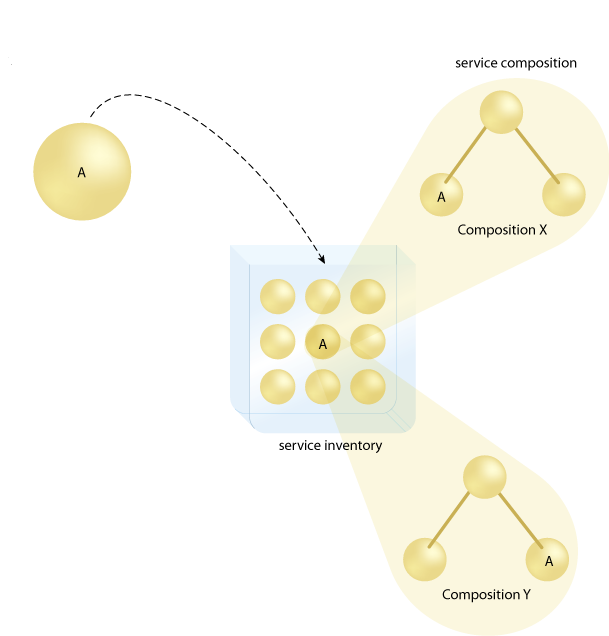
\includegraphics[width=0.4\textwidth]{images/picservi0}
	\caption{Service inventory\cite{picservi}}
	\label{fig:Serviceinventory}
	\end{figure}
	\FloatBarrier \noindent
\textbf{Orchestration}\\
Orchestration means, that a new Service can be build out of other Services which are in the service inventory, as it can be seen in figure \ref{fig:Serviceinventory}. \\
These other services can be of any kind (also external) and the communication between them is usually coordinated out from an central controlling instance. Orchestration is usually done using (WS-)BPEL. This layer is also a reason why \gls{soa} is so flexible and why the systems must be loosely coupled. \cite[page 29]{soagoesreal}\\ \\
It therefore helps to produce code out of a graphical description, and there is no need to code it all out once again. Such systems should interact with other systems such as \gls{erp}-systems and without \gls{soa} it would be hard to realize. Using BPEL, smaller parts of an application can be easily combined to a greater one. \cite[page 18]{soagoesreal} \\ \\
\\
%\begin{figure}[here!]
%	\centering
%	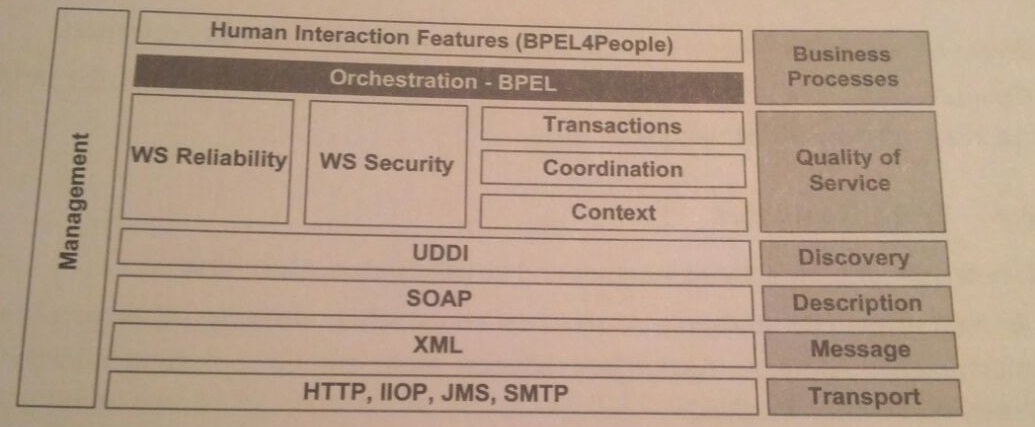
\includegraphics[width=0.6\textwidth]{images/page19}
%	\caption{BPEL as orchestration layer \cite[page 19]{soagoesreal}}
%	\label{fig:bpel}
%	\end{figure}
%	\FloatBarrier
\subsection{SOA Model}
The \gls{soa}-model has different layers. On the top level there is the Presentation Layer, which is the User Interface, which can be a normal Client Application as we know it but also a Fat Client. Then we speak of the Orchestration Layer, Where the flow of an Application is beeing a sequence of certain services. In the Orchestration layer, a data transfer between these Services is possible as well. And then there comes the service layer, in which the Services are. In between there is some kind of integration Architecture, which would normally be an \gls{esb}. In the application layer, applications that already exists and Databases or systems are put. In the Visualized Infrastructure, the Hardware can be found. %These layers can be seen in figure \ref{fig:soamodelarch}.\\
\newpage\noindent\textbf{SOA models}\\
There exist different SOA models, such as the OASIS model, The SOA Meta model of the W3C and each of the bigger companies such as IBM, SAP or Oracle have their own interpretation.
\subsubsection{The SOA Triangle}
\label{sec:soatriangle}
The \gls{soa} triangle (figure \ref{fig:servicetri} \& \ref{fig:comtri}) is consists of three parts:
\\\\\textbf{The Service consumer} \\
This is bascially the client, which wants to use a specific service. It is requesting the Service Registry 	for the address of the specific service he wants to access. He is using the Interface Definition Language in order to  access the Service provider in the right way.
\\\\\textbf{The Service provider}\\ 
This is the part of the system, which is providing some kind of service to a costumer. It is publishing / registering itself in the SOA registry. For this purpose, WSDL is used.
\\\\\textbf{The registry}\\ 
"An SOA registry is a resource that provides controlled access to data necessary for governance of SOA (service-oriented architecture) projects. In effect, it is a constantly evolving catalog of information about the available services in an SOA implementation. An SOA registry allows businesses to efficiently discover and communicate with each other using Web services. The ultimate goal is to allow fast and reliable communication and interoperability among diverse applications with minimal human oversight.", \cite{soareg}\\
The registry's task is it therefore to know the metadata and the addresses of the services and discovery / find the right service provider when a service consumer makes a request.
The UDDI standard is used for locating a service in the registry.

\begin{figure}[here!]
\centering
\begin{minipage}[h]{0.4\textwidth}
\centering
    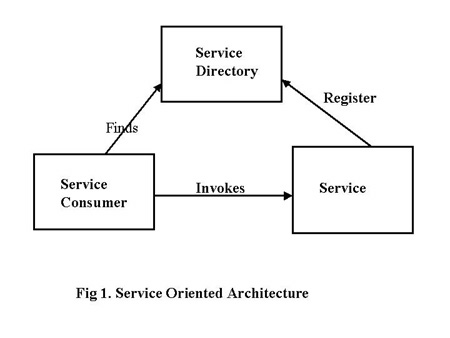
\includegraphics[width=1.0\textwidth]{images/arg3}
    \caption{SOA's components \cite{arg3}}
    \label{fig:servicetri}
\end{minipage}
\begin{minipage}[h]{0.19\textwidth}
\vfill
\end{minipage}
\begin{minipage}[h]{0.4\textwidth}
\centering
    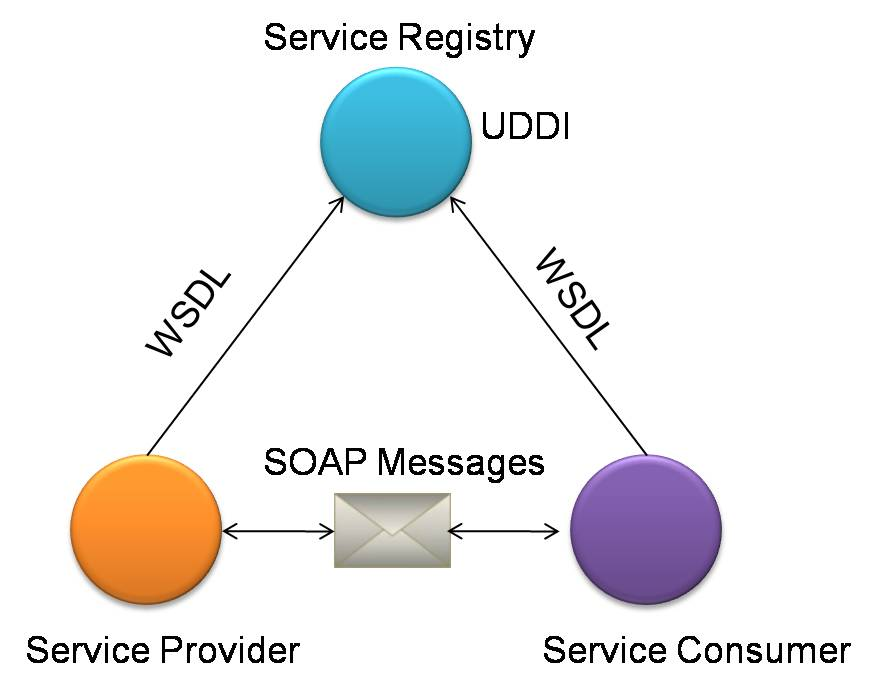
\includegraphics[width=1.0\textwidth]{images/arg1}
    \caption{Communication protocols between components \cite{arg1}}
    \label{fig:comtri}
\end{minipage}
\end{figure}
\FloatBarrier

%\section{JAX-WS}
%SOAP-based Web services support in Java EE 5,6 and 7 is based on the Java API ....
%site 112 grey book 

\newpage

\section{Implementation}
\subsection{ESB}
\label{sec:esb}
\textbf{Possible communication ways between applications} \\ \\
\textit{Peer-to-peer - topology}\\
The peer-to-peer (Figure \ref{fig:eai0}) implementation is not very useful. It is quite outdated and it is not really usable for modern systems.
There is practically no way to achieve any scalability and it gets complicated very soon. \\\\
\textit{Hub \& Spoke  - topology}\\
Messages get directed to an centralized unit, where they can be processed. (Figure \ref{fig:eai1}) This centralized unit can be a bottleneck though. \\\\
\textit{Bus - topology}\\
Every service is connected to an service bus (\gls{esb}).(Figure \ref{fig:eai2}) The processing distribution in this case is very good. The bus-topology is therefore the most recommended one, because there is no bottleneck when comparing it to a Hub.
\begin{figure}[here!]
\centering
\begin{minipage}[h]{0.3\textwidth}
\centering
    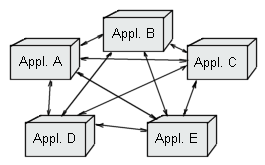
\includegraphics[width=1.0\textwidth]{images/eai0.png}
    \caption{Star \cite{thorstenhorn}}
    \label{fig:eai0}
\end{minipage}
\begin{minipage}[h]{0.3\textwidth}
\centering
    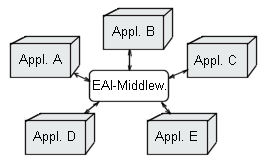
\includegraphics[width=1.0\textwidth]{images/eai1.png}
    \caption{Hub \cite{thorstenhorn}}
    \label{fig:eai1}
\end{minipage}
\begin{minipage}[h]{0.3\textwidth}
\centering
    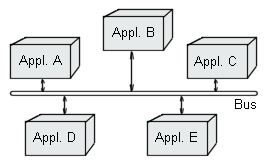
\includegraphics[width=1.0\textwidth]{images/eai2.png}
    \caption{Bus \cite{thorstenhorn}}
    \label{fig:eai2}
\end{minipage}
\end{figure}
\FloatBarrier  \noindent
\textbf{Enterprise Service Bus} \\
"An enterprise service bus (ESB) is a software architecture for middleware that provides fundamental services for more complex architectures. [..] . In a general sense, an ESB can be thought of as a mechanism that manages access to applications and services (especially legacy versions) to present a single, simple, and consistent interface to end-users via Web- or forms-based client-side front ends.", \cite{esbdef}\\
Its main task are to:
\begin{itemize}
\item Distribute information across an enterprise quickly and easily
\item Identify Messages and route them between services
\item Mask differences among underlying platforms, software architectures, message formats and network protocols as they move from service requestor to service provider and back
\item Ensure information delivery even when some systems or networks may go off-line from time to time.
\item Re-route, log, and enrich information without requiring applications to be rewritten.
\item Manages descriptions and definitions of messages and their formats through metadata
\item Creates an extensible architecture based on pluggable components
\end{itemize} \cite{esbdef,esbimplpatt} \\
An ESB has is also not a concrete implementation. Mostly, big companies (e.g. IBM, SAP, TIBCO, Orcale ,..) offer ESB implementations, but there are also open source ones, such as openESB for example.

\textbf{Special routing and transformation} \\
An \gls{esb} also offers content (figure \ref{fig:content}) % and context (figure \ref{fig:context}) 
based  routing and message transformation (figure \ref{fig:Datafromtrans}).\\\\
First of all, content based routing is routing the message based on its content and not on a destination. By looking into the message and deciding which service might be interested in the message, a high degree of flexibility and scalability is achieved.\\ %With the context based routing, the message is simply transferred the normal way.
\\The esb can also do an data format transformation, with might output the data just the way a service wants to have it.

%\begin{figure}[here!]
%	\centering
%	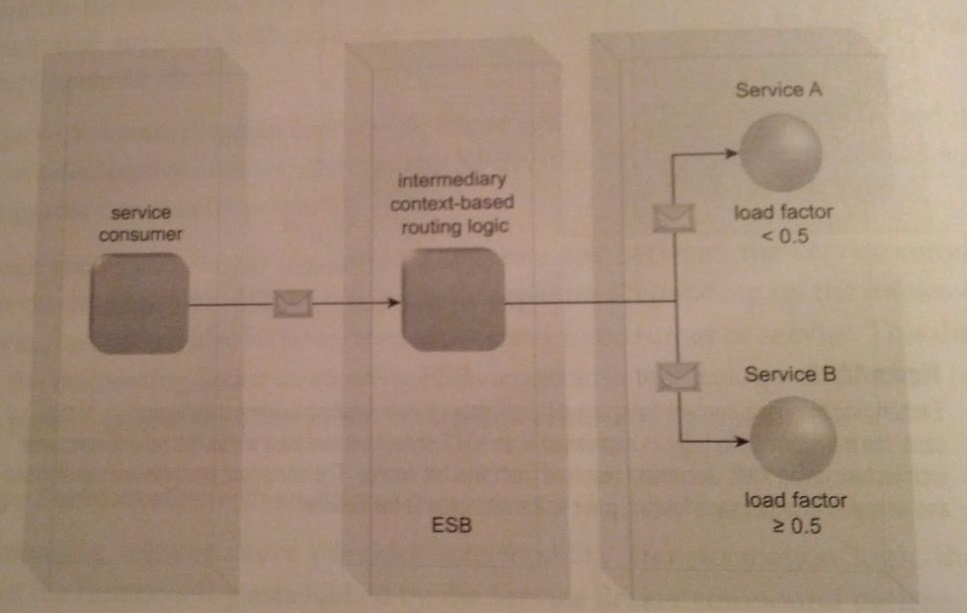
\includegraphics[width=0.5\textwidth]{images/context}
%	  \caption{Context based routing within an \gls{esb} \cite[page 394]{grau}\\This means, the routing is done over load}
%    \label{fig:context}
%	\end{figure}
%	\FloatBarrier
	
	\begin{figure}[here!]
	\centering
	  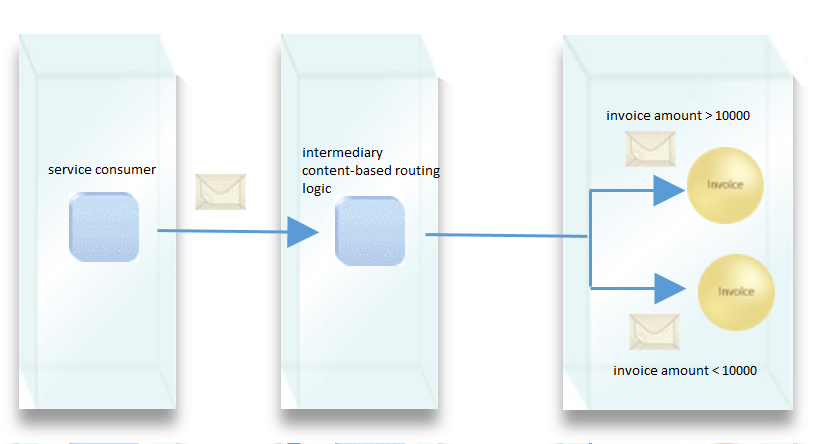
\includegraphics[width=0.6\textwidth]{images/esb123}
	   \caption{Content based routing within an \gls{esb} \\ (\cite[page 394]{grau}, Hannah Siegel)}
    \label{fig:content}
	\end{figure}
	\FloatBarrier
\noindent

\begin{figure}[here!]
	\centering
	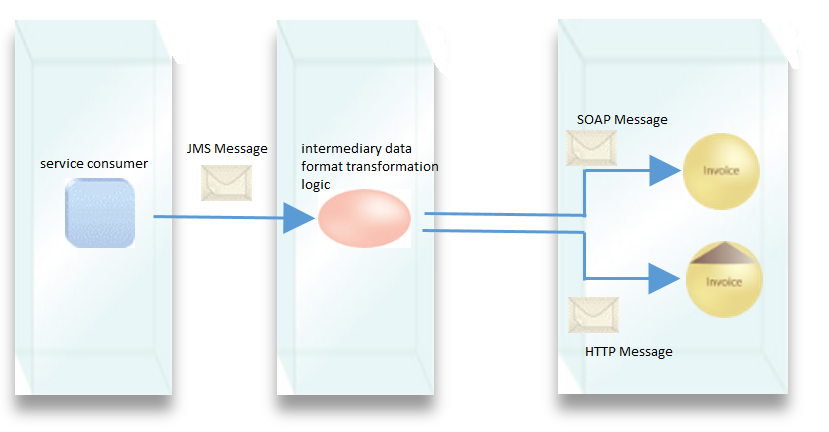
\includegraphics[width=0.6\textwidth]{images/esb456}
	\caption{\gls{esb} carrying out data transformation \\ (\cite[page 395]{grau}, Hannah Siegel)}
\label{fig:Datafromtrans}
	\end{figure}
	\FloatBarrier
\noindent
	
	
	
	
%\begin{figure}[here!]
%	\centering
%	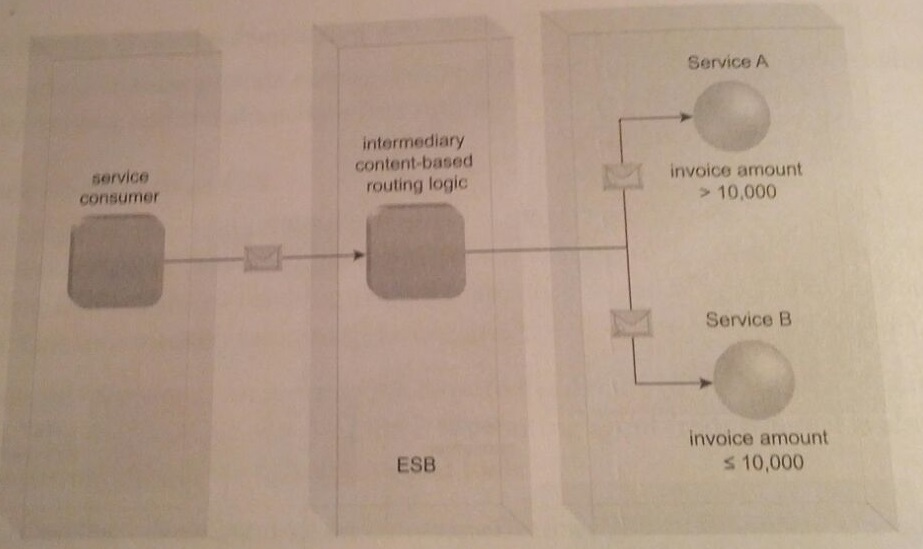
\includegraphics[width=0.5\textwidth]{images/content}
%	   \caption{Content based routing within an \gls{esb} \cite[page 394]{grau}}
%    \label{fig:content}
%	\end{figure}
%	\FloatBarrier


%\begin{figure}[here!]
%	\centering
%	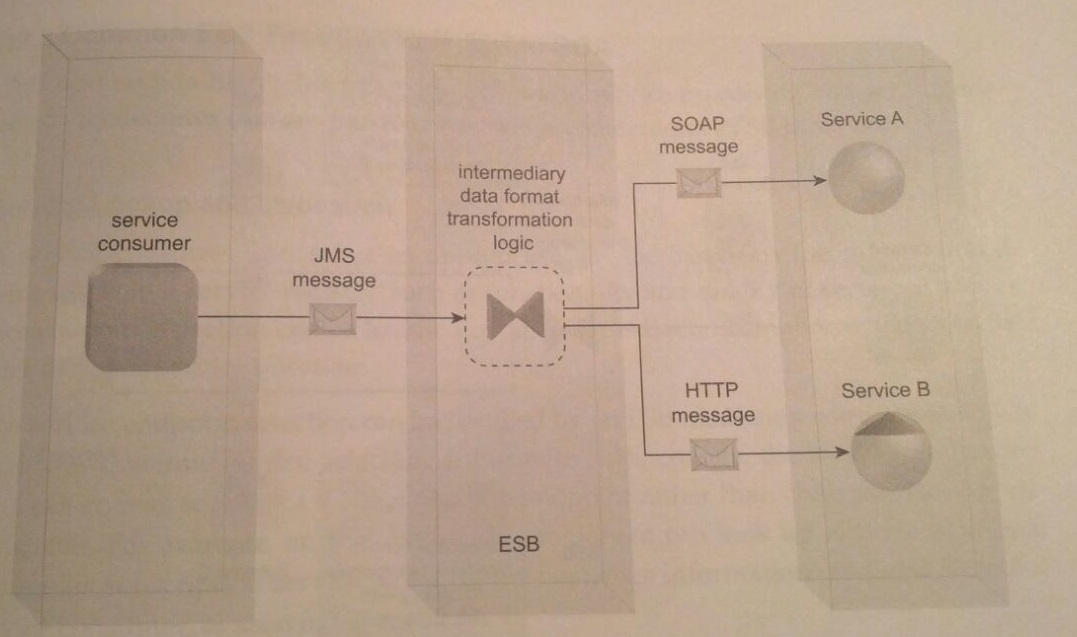
\includegraphics[width=0.5\textwidth]{images/page395}
%	\caption{\gls{esb} carrying out data transformation \cite[page 395]{grau}}
%	\label{fig:Datafromtrans}
%	\end{figure}
	\FloatBarrier
\subsubsection{OpenESB}
"OpenESB is a Java based open source enterprise service bus. It can be used as a platform for both Enterprise Application Integration and Service Oriented Application. OpenESB allows you to integrate legacy systems external and internal partners and new developments in your Business Process.  OpenESB is the unique open source ESB relying on standards that provides you with Simplicity, Efficiency, Long term durability, save on your present and future investments with a very low TCO (Total Cost of Ownership).", \cite{Aboutopenesb}


\subsection{RestFul Web Services}
RESTful web services are built to work best on the Web. RESTful applications use HTTP requests to post data (create and/or update), read data (e.g., make queries), and delete data. Thus, REST uses HTTP for all four CRUD (Create/Read/Update/Delete) operations. If you want to access resources like data and functionallaty in the REST architectural style you have to use Uniform Resource Identifiers which are typicaly links 
on the Web. The REST architectural style constrains an architecture to a client/server architecture and is designed to use a stateless communication protocol, typically HTTP. In the REST architecture style, clients and servers exchange representations of resources by using a standardized interface and protocol. \\
The following principles encourage RESTful applications to be simple, lightweight, and fast:
\\
\begin{itemize}
\item Resource identification through URI: 
A RESTful web service exposes a set of resources that identify the targets of the interaction with its clients. Resources are identified by URIs, which provide a global addressing space for resource and service discovery.\\
\item Uniform interface: 
Resources are manipulated using a fixed set of four create, read, update, delete operations: PUT, GET, POST, and DELETE. PUT creates a new resource, which can be then deleted by using DELETE. GET retrieves the current state of a resource in some representation. POST transfers a new state onto a resource.\\
\item Self-descriptive messages: 
Resources are decoupled from their representation so that their content can be accessed in a variety of formats, such as HTML, XML, plain text, PDF, JPEG, JSON, and others. Metadata about the resource is available and used, for example, to control caching, detect transmission errors, negotiate the appropriate representation format, and perform authentication or access control. \\
\item Stateful interactions through hyperlinks:
Every interaction with a resource is stateless; that is, request messages are self-contained. Stateful interactions are based on the concept of explicit state transfer. Several techniques exist to exchange state, such as URI rewriting, cookies, and hidden form fields. State can be embedded in response messages to point to valid future states of the interaction.\\
\end{itemize}
HTTP Verbs:
\begin{itemize}
\item GET\\
The HTTP GET method is used to retrieve (or read) a representation of a resource.
\item PUT\\
PUT is most-often utilized for update capabilities.
\item POST\\
The POST verb is most-often utilized for creation of new resources.
\item DELETE\\
DELETE is used to delete a resource identified by a URI.
\end{itemize}
\cite{RESTful}

%TODO use the esb chapter
\subsection{Migration of legacy systems}
SOA is steadily becoming mainstream software engineering practice. Reports show that more than 50 percent of large, newly developed applications and business processes designed during the year 2007 used service-oriented architectures to some extent. However, experience also indicates that SOA initiatives rarely start from scratch. The technology market research firm Gartner estimates that by 2011 (with 0.8 probability) more than 80 percent of existing applications will be at least partly reengineered to participate in service-oriented architectures . This represents a significant effort for IT departments of organisations.Because it has characteristics of loose coupling, published interfaces, and a standard communication model, SOA enables existing legacy systems to expose their functionality as services, presumably without making significant changes to the legacy systems. Migration of legacy systems to service-oriented environments has been achieved within a number of domains, showing that the promise is beginning to be fulfilled.\cite{legacy}.
\\
\subsection{Communication Standards}

\subsubsection{XML}
XML stands for EXtensible Markup Language.XML was designed to describe data.
It is a software- and hardware-independent tool for carrying information.\\
Besides HTML and XHTML the most widespread RESTful HTTP-enviroment.\\
Nearly all other standards originate from XML.
\subsubsection{JSON}
JSON is a syntax for storing and exchanging data.The focus here lies in datastructure and not text.
It does not support namespaces and schemed based validation but is easier to understand than XML.
\subsubsection{SOAP}
SOAP was originally a shortcut for "Simple Object Access Protocol", but since it isn't simple 
and it isn't used to access object only the protocol was correct. Since version 1.2 the shortcut
was abolished and SOAP now stands for itself. SOAP is an XML based protocol for accessing Web Services. \\
"Today's applications communicate using Remote Procedure Calls (RPC) between objects like DCOM and CORBA, but HTTP was not designed for this. RPC represents a compatibility and security problem; firewalls and proxy servers will normally block this kind of traffic. A better way to communicate between applications is over HTTP, because HTTP is supported by all Internet browsers and servers. SOAP was created to accomplish this.SOAP provides a way to communicate between applications running on different operating systems, with different technologies and programming languages. A SOAP message is an ordinary XML document containing the following elements:
\begin{itemize}
\item An Envelope element that identifies the XML document as a SOAP message
\item A Header element that contains header information
\item A Body element that contains call and response information
\item A Fault element containing errors and status information"
\end{itemize}
\cite{soap}\\
SOAP envelope structure:\\

\begin{figure}[here!]
	\centering
	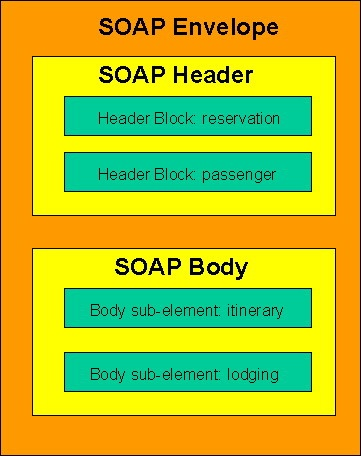
\includegraphics[width=0.3\textwidth]{images/soa_envelope}
	\caption{soapbild}
    \label{fig:Soapenvelope}
	\end{figure}
	\FloatBarrier


	
\subsubsection{WSDL}
Web Service Description Language is a XML based Interface communicationinterface description language
which is used to describe web services which are called by SOAP-Messages.
Currently there are two Versions:\\
1.1 : Which is used Worldwide and is supported by nearly every tool. \\
2.0 : Brings some improvements but they are not relevant in the praxis so this version is not often
used.\\
WSDL describes a Web service. It specifies the location of the service and the operations (or methods) the service exposes.\\
\cite{wsdl}\newpage
\subsubsection{UDDI}
"Universal Description, Discovery and Integration (UDDI) is a directory service where businesses can register and search for Web services.
UDDI is a platform-independent framework for describing services, discovering businesses, and integrating business services by using the Internet.\\
\begin{itemize}
\item UDDI stands for Universal Description, Discovery and Integration
\item UDDI is a directory for storing information about web services
\item UDDI is a directory of web service interfaces described by WSDL
\item UDDI communicates via SOAP
\item UDDI is built into the Microsoft .NET platform
\end{itemize}
UDDI uses World Wide Web Consortium (W3C) and Internet Engineering Task Force (IETF) Internet standards such as XML, HTTP, and DNS protocols.
UDDI uses WSDL to describe interfaces to web services Additionally, cross platform programming features are addressed by adopting SOAP, known as XML Protocol messaging specifications found at the W3C Web site."\cite{uddi}\\
A UDDI WSDL and SOAP example can be found here in here: \ref{fig:eai1}
\section{Code Snippets}
\subsection{JSON vs XML Example}
\label{sec:json}
The following JSON example defines an employees object, with an array of 3 employee records:
\begin{lstlisting}
{{"employees":[
    {"firstName":"John", "lastName":"Doe"}, 
    {"firstName":"Anna", "lastName":"Smith"},
    {"firstName":"Peter", "lastName":"Jones"}
]}
\end{lstlisting}
The following XML example also defines an employees object with 3 employee records:
\begin{lstlisting}
<employees>
    <employee>
        <firstName>John</firstName> <lastName>Doe</lastName>
    </employee>
    <employee>
        <firstName>Anna</firstName> <lastName>Smith</lastName>
    </employee>
    <employee>
        <firstName>Peter</firstName> <lastName>Jones</lastName>
    </employee>
</employees>
\end{lstlisting}
In this example you can see that JSON is easier to understand ,more compact and more readable than JSON.
Also as you can see JSON sends less data so it can be faster in transmissions.\cite{jsonxml}
\subsection{SOAP Example}
\label{sec:soapeexample}
\textbf{SOAP request}\\
\begin{lstlisting}
<?xml version="1.0"?>
<soap:Envelope
xmlns:soap="http://www.w3.org/2001/12/soap-envelope"
soap:encodingStyle="http://www.w3.org/2001/12/soap-encoding">

<soap:Body xmlns:m="http://www.example.org/stock">
  <m:GetStockPrice>
    <m:StockName>IBM</m:StockName>
  </m:GetStockPrice>
</soap:Body>

</soap:Envelope>
\end{lstlisting}
\textbf{SOAP response}
\begin{lstlisting}
<?xml version="1.0"?>
<soap:Envelope
xmlns:soap="http://www.w3.org/2001/12/soap-envelope"
soap:encodingStyle="http://www.w3.org/2001/12/soap-encoding">

<soap:Body xmlns:m="http://www.example.org/stock">
  <m:GetStockPriceResponse>
    <m:Price>34.5</m:Price>
  </m:GetStockPriceResponse>
</soap:Body>

</soap:Envelope>
\end{lstlisting}
In the example above, a GetStockPrice request is sent to a server. The request has a StockName parameter, and a Price parameter that will be returned in the response. The namespace for the function is defined in \texttt{http://www.example.org/stock}.\cite{soap}\\
\newpage
\subsection{WSDL Example}
\label{sec:wsdlexample}
\begin{lstlisting}
<message name="getTermRequest">
  <part name="term" type="xs:string"/>
</message>

<message name="getTermResponse">
  <part name="value" type="xs:string"/>
</message>

<portType name="glossaryTerms">
  <operation name="getTerm">
    <input message="getTermRequest"/>
    <output message="getTermResponse"/>
  </operation>
</portType>
\end{lstlisting}
"In this example the \textless portType\textgreater element defines glossaryTerms as the name of a port, and getTerm as the name of an operation. The getTerm operation has an input message called getTermRequest and an output message called getTermResponse. The \textless message\textgreater elements define the parts of each message and the associated data types.Compared to traditional programming, glossaryTerms is a function library, getTerm is a function with getTermRequest as the input parameter, and getTermResponse as the return parameter."\cite{wsdl}


\section{Comparison and Conclusion}
\subsection{SOA VS. EAI}
\textbf{EAI}\\
With the rise of \gls{eai}, Middleware was introduced and trough Adapters and Brokers with whom the whole IT-infrastructure got manageable. Still, IT-landscapes were still inefficient and continuous change was nearly impossible.\cite[page 115]{te}
\\
\\\textbf{Difference between SOA and EAI}\\
"Differently than EAI, which deals with linking enterprise applications so they can communicate with one another (by means of an intelligent reasoning engine) and carry out 'batch' data transfers, is the service oriented architecture (\gls{soa}) that provides 'transactional' data transfers, with no third-party software required. SOA is different from the EAI approach in that it does not depend on a third-party solution and that it is only providing an design structure and principles." ,\cite{soadef}\\
\\
\gls{soa} therefore emerged out of \gls{eai} as a newer design approach. Still, many companies are using systems such as \gls{eai}, because the change to a service-oriented approach might not always be easy. 
%\subsection{SOA VS. OOP}
%TODO ??
%\subsection{SOA VS. AOP} %TODO weg?
%\textbf{Aspect oriented programming (\gls{aop})}\\
%"An aspect is a common feature that's typically scattered across methods, classes, object hierarchies, or even entire object models. It is behavior that looks and smells like it should have structure, but you can't find a way to express this structure in code with traditional object-oriented techniques.\\
%For example, metrics is one common aspect. To generate useful logs from your application, you have to (often liberally) sprinkle informative messages throughout your code. However, metrics is something that your class or object model really shouldn't be concerned about. After all, metrics is irrelevant to your actual application: it doesn't represent a customer or an account, and it doesn't realize a business rule. It's simply orthogonal.
%\\
%In AOP, a feature like metrics is called a crosscutting concern, as it's a behavior that "cuts" across multiple points in your object models, yet is distinctly different. As a development methodology, AOP recommends that you abstract and encapsulate crosscutting concerns." \cite{aopdef}
%TODO
\subsection{SOAP VS. REST}
Pro and Contra:\\ 
\begin{itemize}
\item One of the major benefits of RESTful API is that it is flexible for data representation, for example you could serialize your data in either XML or JSON format.
\item SOAP on the other hand is the prevailing standard for web services, and hence has better support from other standards (WSDL, WS-*) and tooling from vendors.
\item REST is easier to understand than SOAP and is closer in design and philosophy to the Web, but it is tied to the HTTP transport model and is point-to-point only.
\item SOAP is a bit complexer than REST and only uses XML, but security and authorization are part of the protocol.
\end{itemize}
\textbf{Conclusion REST:}\\
You should use REST when Client and Server operate on a Web environment.\\
You shouldn't use REST When you need to enforce a strict contract between client and server\\
\\\textbf{Conclusion SOAP:}\\
You should use SOAP when when clients need to have access to objects aviable on servers.\\
You shouldn't use SOAP when your bandwidth is very limited.\\
\subsection{Pro and Contra of SOA}
Even trough \gls{soa} provides a very flexible and cost efficient environment, but it might not always be the the best solution.
\\ \\
\textbf{The Good}\\
The reusability for sure is a great advantage of \gls{soa}, if they are designed with the right patterns.
Because services share schemas and contracts, not classes and types, a higher platform neutrality is reached. Avoiding type system dependency is what ensures interoperability. \\
What probably speaks the most for \gls{soa}, is the \gls{roi}, if applied right. This can be seen in figure \ref{fig:roi}: Even trough the delivery cost with \gls{soa} is 30\% higher, the \gls{roi} after 3 years is 3 times higher! Of course, the exact \gls{roi} depends on various impacts, so the values are just an example. \cite{pcsoa}
\begin{figure}[here!]
	\centering
	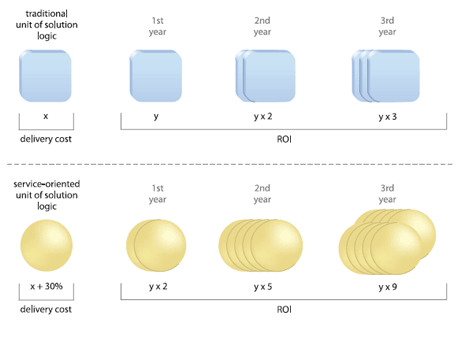
\includegraphics[width=0.5\textwidth]{images/roi}
	\caption{ROI \cite{roiph}}
	\label{fig:roi}
	\end{figure}
 \noindent



%"Service orientation via web services can often be the best approach for enabling core business processes. The most important aspect to finding the SO sweet spot is determining what can be reused. Services are often considered application building blocks. With that comes a great responsibility for the application visionaries. [..] 
%If these services are envisioned and designed with the enterprise in mind, and not the specific application being envisioned, there is a good chance that a reusable service will be delivered. [..] You have to involve the right resources for auditing those services which are thought to be reusable. [..]
%Loosely-coupled, reusable services have a number of other obvious benefits. \\
%Services share schemas and contracts, not classes and types: This speaks to the platform neutrality of services. All services are designed to exchange contracts for behavior and schemas for data structure. Avoiding type system dependency is what ensures interoperability. \\
%Policies define the constraints for accessing the service. This allows services to define a mechanism for communicating no matter what their current capabilities are.\\
%Each of these parts is also individually scalable.\\Services can also see a huge gain in maintainability and extensibility because of their centralized nature.\\ \\
%When you have a need for interoperability, service orientation has obvious benefits. If you need to expose your application’s business logic to a brand new front end hosted on a disparate platform, SOA provides exceptional ROI.
% "\cite{pcsoa} \\ \\
\newpage
\noindent\textbf{The Bad} \\
The performance might not be optimal, but nowadays, performance is less important than it was a few years ago. \\
Because of interoperability, security is more complicated. Also, the tools and know-how available is not exactly great.\\
Quality assurance and testing might be more difficult, because of the complexity involved in the test environment setup. It therefore becomes more challenging to trace application code at runtime and quickly do problem determination on systems that live on numerous servers and sometimes on disparate platforms.
\\
The last problem is that versioning of services. Any behavioural changes to an exposed service can negatively impact consuming applications, because they could  depend on things like error conditions or failure scenarios in previous versions of the service. \cite{pcsoa}







%Even trough the performance of \gls{soa} might not be perfect, it should not be used as a driving factor for deciding whether or not to move toward service orientation, because also based on Moores Law, performance isn't really a thing we need to worry about greatly. \cite{pcsoa}\\
%Interoperable security is very complicated: Both method-level security and role-based security become very challenging to implement when considering interoperability concerns. \\
%\\ \\ 
%The tools available today for service-oriented development are still somewhat unsophisticated.
%\\ \\
%"The most costly aspect of introducing new technologies and concepts is the investment in your company’s human capital. People are resilient and, in some cases, are very agile, but that agility comes with time and experience.",\cite{pcsoa}
%One of the most challenging roles in the service-oriented era is that of the quality assurance engineer. Most services are designed to satisfy the needs of various applications; that makes their requirements somewhat fragmented.
%Another not-so-obvious added cost with service orientation is the complexity involved in the test environment setup.
%Another major problem with versioning of services is any implicit semantic contract changes. Any behavioral changes to an exposed service can negatively impact consuming applications. 
%Consumers could potentially depend on things like error conditions or failure scenarios in previous versions of the service. 
%As with other distributed technologies, it becomes more challenging to trace application code at runtime and quickly do problem determination on systems that live on numerous servers and sometimes on disparate platforms.

\subsection{Conclusion}
Whereas \gls{soa} can not be seen as an implementation but more as an design principle, it comes with many advantages. Using the Web-oriented approach and also putting Services and Business Processes into the focus, it leaves an very flexible IT-Infrastructure and leads to an cost efficient way of operating.\\
Depending on a role in an enterprise, staff will be impacted by \gls{soa} in different ways. It will impact almost everyone responsible for delivering applications. When sticking to the design principles and to the standards, \gls{soa} has the potential to become the best approach for building reusable application landscapes. If not, \gls{soa} may become an infrastructure which may be hard to handle and failing it's original purpose of making things easier and increase the \gls{roi}.\\
Nowadays, many of \gls{soa}'s principles are already used in what we declare as good software design, but still many companies have problems with applying the \gls{soa} Principles at a full extend. Often only parts of it get used, if even. This is mainly because changing an entire infrastructure is not that easy and companies are not always ready for a big change like that. A missing base of know-how or the engineering approach of 'As long as it works, don't change anything' contribute to the fact, that \gls{soa} is not used by every company yet.

%TODO http://serviceorientation.com/soaplanning/fourpillars





\newpage

%\listoftables
\listoffigures
\printglossaries
\begin{thebibliography}{56}

 \bibitem{searchsoa}
   \textbf{service-oriented architecture (SOA) definition},Margaret Rouse \\
  \textit{http://searchsoa.techtarget.com/definition/service-oriented-architecture}
  \newline last used: 03.02.2015, 14:05

\bibitem{grau}
   \textbf{SOA with Java - Realizing Service-Orientation with Java Technologies}\\
   Thomas ERL, Andre TOST, Satadru ROY, Philip THOMAS \\ 
   Prentice Hall \\
   Massachusetts, 2014 \\
	ISBN: 978-0-13-3859003-4 

 \bibitem{soagoesreal}
   \textbf{SOA goes real : Service-orientierte Architekturen erfolgreich planen und einfuehren.}\\
   Daniel LIEBHART \\ 
   Carl Hanser Verlag \\
   Wien, 2007 \\
	ISBN: 978-3-446-41088-6

 \bibitem{patterns}
  \textbf{SOAPatterns.org}, collection of patterns\\
  \textit{http://soapatterns.org/}
  \newline last used : 12.03.2015, 07:18

\bibitem{photos}
  \textbf{Service Orientation .com}, pictures\\
  \textit{http://serviceorientation.com}
  \newline last used : 12.03.2015, 07:12

   \bibitem{soaitwissen}
   \textbf{SOA (service oriented architecture)},IT Wissen \\
  \textit{http://www.itwissen.info/definition/lexikon/service-oriented-architecture-SOA-SOA-Architektur.html}
  \newline last used: 03.02.2015, 13:50

%[7]
   
   	     \bibitem{arg2}
   \textbf{Parts of SOA}, Picture \\
  \textit{http://en.wikipedia.org/wiki/Service-oriented\_architecture -\textgreater Enterprise SOA. Prentice Hall, 2005}
  \newline last used : 11.03.2015, 20:34 	

%[8]
\bibitem{te}
   \textbf{SOA - Entwurfsprinzipien fuer serviceorientierte Architektur}\\
   Thomas ERL\\
   Addison-Wesley \\
   2008 \\
	ISBN: 978-3-8273-2651-5 

\bibitem{json}
  \textbf{JSON},json.com \\
  \textit{http://www.json.org/}
  \newline last used: 02.02.2015, 22:15

  
 
\bibitem{picservi}
   \textbf{Understanding Reuse and Composition: 
Working with the Service Reusability and Service Composability Principles}\\ Thomas Erl, October 12, 2011 \\
  \textit{http://www.servicetechmag.com/i55/1011-3}
  \newline last used: 12.03.2015, 13:39 
 
 
 
 
 %10	 
\bibitem{loosecoupldef}
   \textbf{loose coupling definition}, Margaret Rouse\\
  \textit{ 	 http://searchnetworking.techtarget.com/definition/loose-coupling}
  \newline last used : 10.02.2015, 20:18 	  
  
  
%TODO pasteing


  \bibitem{soamaifesto}
   \textbf{The SOA Manifesto} \\
  \textit{http://www.soa-manifesto.org/default.html}
  \newline last used: 28.02.2015, 14:05
  
 	 
\bibitem{soalycman}
   \textbf{Understanding the SOA lifecycle},  Rich Seeley\\
  \textit{ 	 http://searchsoa.techtarget.com/tip/Understanding-the-SOA-lifecycle}
  \newline last used : 11.03.2015, 12:29 	 
   	    
  
   	  	 
\bibitem{slcmoracle}
   \textbf{Fusion Middleware Concepts and Architecture for Oracle Service Bus}, docs.oracle\\
  \textit{    	  https://docs.oracle.com/cd/E23943\_01/doc.1111/e15020/introduction.htm\#OSBCA107
}
  \newline last used : 08.03.2015, 18:31 	 
  
  
  
\bibitem{bpmdef}
   \textbf{Business Process Management (BPM)}, Margaret Rouse\\
  \textit{http://searchcio.techtarget.com/definition/business-process-management}
  \newline last used : 06.10.2014, 22:13
 
 
 \bibitem{muede2}
   \textbf{What is Business Process Management? }\\
  \textit{http://www.scc-co.com/enterprises-processes/}
  \newline last used : 06.10.2014, 22:04


  \bibitem{bpmchall}
   \textbf{Top Ten Biggest Challenges to BPM Initiatives}, Pearl Zhu\\
  \textit{http://futureofcio.blogspot.co.at/2013/03/top-ten-biggest-challenges-to-bpm.html}
  \newline last used : 06.10.2014, 22:32
   
   
   

\bibitem{thorstenhorn}
   \textbf{Torsten Horn}\newline
  \textit{http://www.torsten-horn.de/techdocs/eai.htm}
  \newline last used : 05.10.2014, 20:25




   	     	  
\bibitem{esbdef}
   \textbf{enterprise service bus (ESB) definition}, Margaret Rouse\\
  \textit{ http://searchsoa.techtarget.com/definition/enterprise-service-bus}
  \newline last used : 08.03.2015, 19:29 	 
   	     	     	     	  



%%%%%%


 
 %weg wenn nicht benuetzt
\bibitem{service1}
   \textbf{Service},service-architecture.com \\
  \textit{http://www.service-architecture.com/articles/web-services/service.html}
  \newline last used: 03.02.2015, 13:39
     
      %weg wenn nicht benuetzt
     \bibitem{soaserviearch}
   \textbf{Service-Oriented Architecture (SOA) Definition},service-architecture.com \\
  \textit{http://www.service-architecture.com/articles/web-services/service-oriented\_architecture\_soa\_definition.html}
  \newline last used: 03.02.2015, 13:40
     
     
  
     
    


     


     \bibitem{bpelsearchsoa}
   \textbf{BPEL (Business Process Execution Language) definition},Margaret Rouse \\
  \textit{http://searchsoa.techtarget.com/definition/BPEL}
  \newline last used: 08.03.2015, 13:21

  \bibitem{legacy}
    \textbf{Migrating Legacy System to Service-Oriented Architecture },Carlos Matos\\
    \textit{http://opus4.kobv.de/opus4-tuberlin/frontdoor/index/index/docId/2999}
    \newline last used : 09.03.2015, 21:50

  \bibitem{RESTful}
    \textbf{What Are RESTful Web Services},Oracle \\
    \textit{http://docs.oracle.com/javaee/6/tutorial/doc/gijqy.html}
    \newline last used : 09.03.2015, 22:30

    \bibitem{uddi}
    \textbf{UDDI },w3school\\
    \textit{http://www.w3schools.com/webservices/ws\_wsdl\_uddi.asp}
    \newline last used : 10.03.2015, 23:55

  


  \bibitem{soadef}
   \textbf{Key differnces between ESB, EAI and SOA}\\
  \textit{www.innovativearchitects.com/KnowloedgeCenter/Business \\ \%20Connectivity\%20and\%20Interoperability/ESB-EAI-SOA.aspx}
  \newline last used : 06.10.2014, 22:18



 	
   	  
\bibitem{bpmldefmr}
   \textbf{Business Process Modeling Language (BPML) definition}, Margaret Rouse\\
  \textit{http://searchsoa.techtarget.com/definition/Business-Process-Modeling-Language-BPML}
  \newline last used : 10.02.2015, 21:09

\bibitem{wsdl}
   	\textbf{WSDL Documentation},w3schools \\
    \textit{http://www.w3schools.com/webservices/ws\_wsdl\_documents.asp}
    \newline last used : 10.03.2015, 23:00

\bibitem{soap}
	\textbf{SOAP Documentation},w3schools \\
    \textit{http://www.w3schools.com/webservices/ws\_soap\_intro.asp}
    \newline last used : 10.03.2015, 23:10  
   	 
   	 
   	 \bibitem{aopdef}
	\textbf{What Is Aspect-Oriented Programming?}, jboss doc \\
    \textit{http://docs.jboss.org/aop/1.1/aspect-framework/userguide/en/html/what.html 	 }
    \newline last used : 10.03.2015, 21:40  
   	 
   	 	 \bibitem{pcsoa}
	\textbf{The Good, the Bad, and the Ugly of Service-Oriented Architecture}, Tom Fuller, 23.08.2005 \\
    \textit{http://aspalliance.com/707\_The\_Good\_the\_Bad\_and\_the\_Ugly\_of\_ServiceOriented\_Architecture.all}
    \newline last used : 11.03.2015, 12:12  
 	 
 	    \bibitem{roiph}
  \textbf{Increasing SOA ROI and maximizing automated solutions}\\
  \textit{ 	 http://searchitchannel.techtarget.com/feature/Increasing-SOA-ROI-and-maximizing-automated-solutions}
  \newline last used : 12.03.2015, 13:08


 	 
   	  

 	     	  
\bibitem{Aboutopenesb}
   \textbf{About OpenESB }, open-esb.net\\
  \textit{http://www.open-esb.net/index.php?option=com\_content\&view=article\&id=104\&Itemid=490}
  \newline last used : 08.03.2015, 19:56 	 
   	     	     	     	     	     	     	     	  
   	     
\bibitem{esbimplpatt}
   \textbf{Enterprise Service Bus implementation patterns} \\ Victor Grund,Chuck Rexroad , 05.12.2007, ibm.com\\
  \textit{ http://www.ibm.com/developerworks/websphere/library/techarticles/0712\_grund/0712\_grund.html}
  \newline last used : 08.03.2015, 20:12 	   	     
   	     	     	     	 
 	    	     
\bibitem{arg1}
   \textbf{Role of Web Services in SOA} \\
  \textit{ 	 http://blog.krawler.com/2009/08/role-of-web-services-in-soa/}
  \newline last used : 08.03.2015, 20:12 	   	     
   	     	     	     	 
   	  
     	     	     	 
  \bibitem{arg3}
   \textbf{What is SOA?}, onjava.com \\
  \textit{http://www.onjava.com/2005/01/26/soa-intro.html}
  \newline last used : 11.03.2015, 20:35
 	 
 	 
 	 \bibitem{soareg}
   \textbf{SOA registry definition}, Margaret Rouse\\
  \textit{http://searchsoa.techtarget.com/definition/SOA-registry}
  \newline last used : 11.03.2015, 20:44 	 
   	     	   
   	 \bibitem{soaprov}
   \textbf{SOA in Practice The Art of Distributed System Design}\\
   Nicolai M. Josuttis\\
   dpunkt Verlag \\
   Heidelberg,2008 \\
	ISBN: 978-3-89864-476-1

  \bibitem{resthttp}
  \textbf{REST und HTTP}\\
   Stefan Tilkov\\
   dpunkt Verlag \\
   Heidelberg,2009 \\
	ISBN: 978-3-89864-583-6

 \bibitem{javawebservice}
  \textbf{Java Web Services in der Praxis}\\
  Oliver Heuser and Andreas Holubek\\
  dpunkt Verlag \\
  Heidelberg 2010 \\
	ISBN: 978-3-89864-596-6

   \bibitem{restcookbook}
  \textbf{RESTful Web Services Cookbook}\\
   Subbu Allamaraju\\
   O'REILLY \\
   2011 \\
	ISBN: 978-0-596-80168-7

  \bibitem{jsonxml}
  \textbf{JSON Tutorial},W3Schools\\
  \textit{http://www.w3schools.com/json/}
  \newline last used : 12.03.2015, 11:45
  
  \bibitem{soapbild}
  \textbf{Nachrichten verschicken mit SOAP - Die SOAP-Spezifikation},02.02.2007, von Dr. Klaus Manhart\\
  \textit{http://www.tecchannel.de/webtechnik/soa/458074/nachrichten\_verschicken\_mit\_soap\_die\_soap\_spezifikation/index4.html
}
  \newline last used : 12.03.2015, 11:45



 	 
 	 
\end{thebibliography}
\end{document}
